\begin{pastexam}[label={px:ncku-113-ee-18}]{成大電機所 113 學年度 簡答題第 9 題}
（簡答）

(5 pts) We can search a number by rank in a binary search tree if we add an additional
information to each node. Please show the number of comparisons before we can find the 4-th
smallest values in the right tree and give the information of each node to complete the
procedure.

\begin{center}
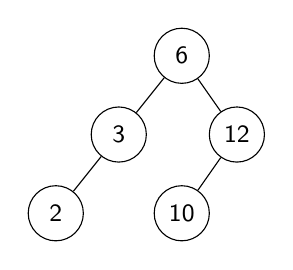
\begin{tikzpicture}[v/.style={draw,circle,minimum size=0.7cm,inner sep=0pt,font=\sffamily\small}]
  \node[v] (6) at (0,0) {6};
  \node[v] (3) at (-0.8,-1) {3};
  \node[v] (12) at (0.7,-1) {12};
  \node[v] (2) at (-1.6,-2) {2};
  \node[v] (10) at (0,-2) {10};
  \draw (6)--(3) (6)--(12) (3)--(2) (12)--(10);
\end{tikzpicture}
\end{center}
\end{pastexam}

\begin{pastsoln}
這份考卷和成大電通所 113 學年度的「資料結構」是同一份（電機系、電通所、智慧資安學程共用），完整詳解見歷屆試題~\ref{px:ncku-113-cce-18}。

答案：每個節點記子樹大小（$6\colon 5$、$3\colon 2$、$12\colon 2$、$2\colon 1$、$10\colon 1$）；第 $4$ 小是 $10$，走過 $6$、$12$、$10$，共 $3$ 次比較。
\end{pastsoln}
